%%%%%%%%%%%%%%%%%%%%%%%%%%%%%%%%%%%%%%%%%%%%%%%%%%
%                                                %
% Aston University Postgraduate Thesis Template  %
% Author:  Dr Chloe M. Barnes                    %
%          Department of Computer Science        %
%          Aston University                      %
% Version: v1.0                                  %
% Date:    4th May 2023                          %
%                                                %
%%%%%%%%%%%%%%%%%%%%%%%%%%%%%%%%%%%%%%%%%%%%%%%%%%

\documentclass[thesisdraft]{thesis-aston}

%%%%%%%%%% SPECIFICATIONS %%%%%%%%%%

% This template has been altered to incorporate the 
% https://www.aston.ac.uk/system/files/2022-08/Summary%20of%20changes%20to%20Research%20Regulations%20for%202021-22.pdf
\RequirePackage{thesis-aston} % uses the thesis-aston.sty file -- do not remove
% CLASS OPTION: use the `thesisdraft' class option to bring up statistics on the final page about comments left to address

%%%%%%%%%% Non-Essential Packages %%%%%%%%%%

\usepackage{lipsum} % to generate dummy text for the template
\setlength{\marginparwidth}{2cm} % sets margin for notes
\usepackage{todonotes} % enables comment bubbles for todo notes

\usepackage{siunitx} % for formatting scientific numbers (recommended as it makes rounding/changing how numbers are displayed easier)
\usepackage{hyperref} % styles hyperlinks (recommended)
\makeatletter\let\@bibitem\saved@bibitem\makeatother
    \hypersetup{
        colorlinks=false, % link is a box, link is coloured instead if true
        linkcolor=black,  % document links
        citecolor=black,  % bibliography
        filecolor=black,  % links to files
        urlcolor=black    % urls
    }

% Bibliography style commands: these are the recommended values for referencing, however your discipline may require alternative referencing styles. If so, specify here
\RequirePackage[numbers]{natbib}
\bibliographystyle{abbrvnat}

%%%%%%%%%% Author Information %%%%%%%%%%

% Full name: Include all middle names if any
\fullname{Your Full Name}

% Initials: Include all initials with a full-stop after each, as well as lastname. IMPORTANT: add a tilde (~) between each initial/last name, as this provides the correct spacing and not the larger space that usually follows a fullstop
\initials{Y.~F.~Name}

% Month: The month of submission
\thesismonth{April}

% Year: The year of submission
\thesisyear{2023}

% Formatted Thesis Title: Include your thesis title here. Line breaks can be used to format the title in a visually appealling way, such as the example below
\thesistitle{Title of Your Thesis\\You Can Use Breaks\\To Separate It}

% Formatted Thesis Sub-Title: Include your thesis sub-title here. Line breaks can be used to format the title in a visually appealling way, such as the example below. If a sub-title isn't used, leave {} blank
\thesissubtitle{Sub-Title of Your Thesis\\You Can Use Breaks\\To Separate It}
%\thesissubtitle{}

% Thesis Volume: If your thesis comprises more than one volume, specify the volume number here. If this does not apply, leave as 0. This will update the title page
\thesisvolume{1}

% Thesis Type: Specifies your degree programme. 0 --> PhD. 1 --> MSc. 2 --> MA. 3 --> MPhil. 4 --> MD. 5 --> DBA. 6 --> DOptom. 
\thesistype{0}

% Specify page numbering: if true, the front matter pages will be numbered with roman numerals; if false, the title page will start from page 1
%\RomanNumeralsfalse 
% or
\RomanNumeralstrue

%%%%%%%%%% Comment Counters %%%%%%%%%%
% PLEASE READ: 

% Comment counters are an optional addition to this template. You can add both in-line and margin comments, and also personalise comments for the author and add more for supervisors if needed by duplicating the commands.

% To use comment counters, three things need to be changed if changing the command names or adding more:
        % Set up the counters (below)
        % Remove the comment word count from the total word count (below the counter setup)
        % Display the final count (thesis-statistics)
        
\newcounter{comSide}
\newcommand{\comSide}[1]{\stepcounter{comSide}%
    \todo[linecolor=black,backgroundcolor=yellow!30,bordercolor=orange,size=\scriptsize]{Comment: #1}}

\newcounter{comPage}
\newcommand{\comPage}[1]{\stepcounter{comPage}%    
    \todo[inline,linecolor=black,backgroundcolor=yellow!30,bordercolor=orange,size=\scriptsize]{Comment: #1}}

% These commands remove the todos from the word count, keep as comments
% Change the comment commands to your own if needed, or add more for any others you add
%TC:macro \comSide 1
%TC:macro \comPage 1

\begin{document}

%%%%%%%%%% Include Chapters %%%%%%%%%%
% Add a new file for each additional chapter, and add a corresponding \input command to add to the PDF

\begin{thesisfrontmatter}
% Create the title page using the author information specified above
\begin{thesisabstract}[Here, Is, A List, Of, Keywords, You Should Include, Up to, Ten, Separated by, Commas]

Write your abstract here. The \texttt{thesisabstract} environment will automatically format it according to the regulations and give the chapter a title. 

The thesis abstract is a concise description of the work 
undertaken and should contain reference to the problem to be 
addressed, the approach taken, the key results and conclusion. It must 
be written in English. All the information 
should be contained on one sheet of A4 paper unless two abstracts are required (see last sentence). The abstract itself should not exceed 300 words. If the student has obtained permission to submit the thesis in a foreign 
language, a translation of the abstract should also be provided.

\end{thesisabstract}

%%%%%%%%%% DEDICATION (OPTIONAL) %%%%%%%%%%
\begin{thesisdedication}

    Write your dedication here, if you choose to include one, or delete this section.\\

\end{thesisdedication}

%%%%%%%%%% PERSONAL ACKNOWLEDGEMENTS (OPTIONAL) %%%%%%%%%%
\begin{thesisacknowledgements}[0]

Write your personal acknowledgements here, if you choose to include any, or delete this section.

Any collaborative work must be clearly acknowledged by the student in a signed statement submitted with the thesis and this acknowledgement should be included with any others on this page.

\end{thesisacknowledgements}

%%%%%%%%%% COLLABORATOR ACKNOWLEDGEMENTS (OPTIONAL) %%%%%%%%%%
\begin{thesisacknowledgements}[1]

Write your collaborator acknowledgements here, if you choose to include any, or delete this section.

Any collaborative work must be clearly acknowledged by the student in a signed statement submitted with the thesis and this acknowledgement should be included with any others on this page.

\end{thesisacknowledgements}

%%%%%%%%%% PUBLICATIONS (OPTIONAL) %%%%%%%%%%
% List your publications in a manual order using the \publication command.
% If you do not have any publications, feel free to remove the text below
% The \texttt{publicationtype} environment is optional -- this is for if you would like to distinguish between publications arising from your studies, and those that are not as a result of the thesis.

\begin{publications}
    \begin{publicationtype}[0] % Thesis publications 
        \publication{Barnes2019CHARIOTTestbed}
        \publication{Barnes2019saso}
        \publication{Barnes2019SISSY} 
        \publication{Barnes2020CoevolutionaryTasks} 
        \publication{Barnes2020BeyondAgents}
    \end{publicationtype}
    \begin{publicationtype}[1] % Other publications
        \publication{Ghouri2020AAgents}
        \publication{Robinson2021CentralisedAgents}
    \end{publicationtype}
\end{publications}


%%%%%%%%%% Table of Contents, Figures, and Tables %%%%%%%%%%
% These are populated automatically
% If you require additional lists, such as for abbreviations, please add them below    
    \tableofcontents
    \listoffigures
    \listoftables

\end{thesisfrontmatter} % Includes title page, abstract, dedication, acknowledgements, and tables of contents, figures and tables
\chapter{Introduction}\label{chap:intro}

This is an example of how to use a margin comment.\comSide{This is a margin comment} If you wanted to add an in-line comment, you can use the following: \comPage{This is an inline comment.} Then you can carry on with normal text.\\


\noindent You can add quotes like this to your text:
\begin{quote}
The Quote environment is usually for short quotes.
\end{quote}

If you wanted something more lengthy, you can use the Quotation environment, as this keeps the indentation consistent:

\begin{quotation}
The Quotation environment can be used for longer quotes or passages of text. This is formatted differently to the Quote environment, as that does not indent the beginning of the quotation. The Quotation environment also has consistent indentation throughout.
\end{quotation}
\chapter{This Literature Review Title is Very Long but You Can Shorten the Version Displayed at the Top of the Page} 

% This is the short version of the chapter title that will be displayed at the top of the pages
\chaptermark{Literature Review}\label{chap:lit-rev}

\lipsum[1]
\chapter{A Section Name}\chaptermark{Short Version for Top of Page}\label{chap:a section}

% This is an example of how to include published works based on the work in a given chapter. If this is not relevant, please omit.
%%%%%%%%%% Listing Publications at the Start of a Chapter %%%%%%%%%%
% Below are instructions on how to use the environment to list publications. An example of use can be found in a_chapter.tex

% Environment to add text/citations for un/published paper/s at the beginning of the chapter. The environment takes one argument -- specifying how many papers have been PUBLISHED. Use [1] for ONE published paper and any number of unpublished papers, use [2] for TWO OR MORE published papers and any number of unpublished papers, and use [0] for ZERO published papers and ONE OR MORE unpublished papers.

% Usage: 
% \begin{chapter-publications}[2]
% \chappub{Barnes2019saso} % This is the name of the bibtex entry you want to include
% \chappub{Barnes2020BeyondAgents}
% \chapnotpub{Part of this chapter has also been submitted for publication at X.} % This is an unpublished entry. Supply any text as needed
% \end{chapter-publications}

% Alternatively, if not published anywhere but submitted for example:
% \begin{chapter-publications}[0]
% \chapnotpub{The work presented in this chapter has been adapted from work submitted for publication at X.}
% \end{chapter-publications}
%%%%%%%%%%
\begin{chapter-publications}[2]
\chappub{Barnes2019saso}
\chappub{Barnes2020BeyondAgents}
\chapnotpub{Part of the work in this chapter is under review at Journal Name.}
\end{chapter-publications}


\section{Section 1}

\lipsum[1]

		\begin{figure}
    	\centering
    	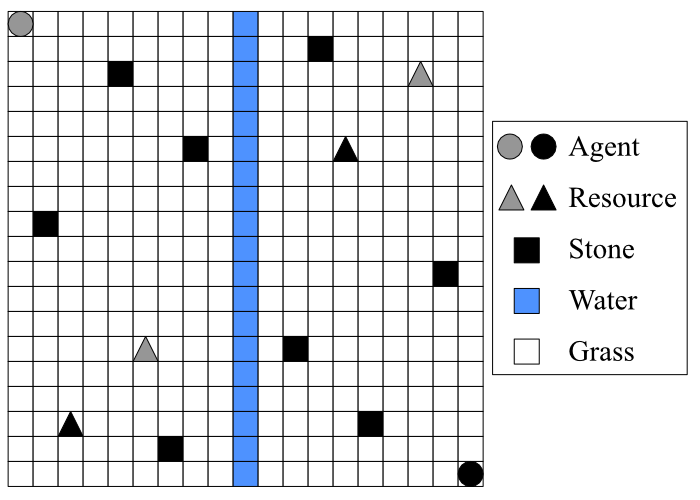
\includegraphics[width=0.75\linewidth]{figures/rcd.png}
    	\caption[The River Crossing Dilemma testbed -- a 2D grid-world environment with a river of Water that agents must cross to retrieve their reward object (Resource).]{The River Crossing Dilemma testbed, which is a 2D grid-world environment. The grey agent (top left) is allocated the two Resources in grey, and the black agent (bottom right) is allocated the two Resources in black; agents cannot interact with Resources that are not allocated to them. Both agents can interact with all other objects. For single-agent environments, the black agent is removed. Figure taken as an example from~\citep{Barnes2021thesis}.}
    	\label{fig: rcd}
	\end{figure}

\lipsum[1]
 
    \begin{figure}
      \centering
      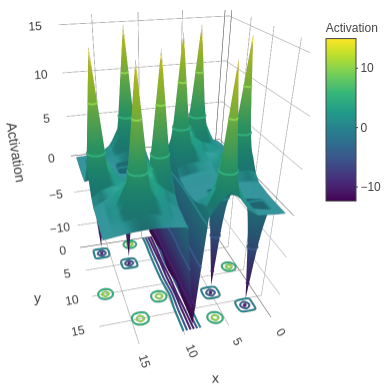
\includegraphics[width=0.5\textwidth]{figures/landscape.png}
      \caption[The reactive network, which generates dynamic activity landscapes that agents use to hill-climb towards their current sub-goals.]{The reactive network generates dynamic activity landscapes with Equation~\ref{eq:shunting equation}, based on the current sub-goals generated by the deliberative network; here, the sub-goals are $[-1,1,-1]$, meaning the agent is attracted to Stones, and avoids Resources and Water. The activity landscape maps to the physical landscape (Figure \ref{fig: rcd}), so agents can hill-climb towards their sub-goals whilst avoiding repulsive objects, by traversing the activity landscape and moving to the adjacent cell with the highest value. Figure taken as an example from~\citep{Barnes2021thesis}.}
      \label{fig: activation landscape}
   \end{figure}
	 
	
	
\section{Another Section}

\lipsum[1] 
    
    An equation here:

    \begin{equation}\label{eq:shunting equation}
        \frac{dx_i}{dt} = -Ax_i + I_i + \sum_{j = 1}^{k} w_{ij}[x_j]^+
        \end{equation}



\section{Using Captioned Sub-Figures}

When using a figure with sub-figures, you can reference individual images such as Figure~\ref{subfig: c}, or the entire figure such as Figure~\ref{fig: some figures}. You can also add \textbf{footnotes}\footnote{Here is an example of a footnote that is formatted correctly, with the correct line spacing and the correct font size.} like this.


    \begin{figure*} 
        \centering
      \subfloat[Caption A \label{subfig: a}
      ]{%
           \includegraphics[width=0.485\linewidth]{example-image-a}}
        \hfill
      \subfloat[Caption B \label{subfig: b}]{%
            \includegraphics[width=0.485\linewidth]{example-image-b}}
        \\
      \subfloat[Caption C \label{subfig: c}]{%
            \includegraphics[width=0.485\linewidth]{example-image-c}}
        \hfill
      \subfloat[Caption D \label{subfig: d}]{%
            \includegraphics[width=0.485\linewidth]{example-image-a}}
        \\
      \subfloat[Caption E \label{subfig: e}]{%
            \includegraphics[width=0.485\linewidth]{example-image-b}}
        \hfill
      \subfloat[Caption F \label{subfig: f}]{%
            \includegraphics[width=0.485\linewidth]{example-image-c}}            
      \caption[A shorter caption. ENSURE ALL FIGURES AND TABLES HAVE A SHORT CAPTION. Do not put references in the short caption, as this forces references to jump to the top of the references list unintentionally.]{A figure containing a number of sub-figures.}
      \label{fig: some figures} 
    \end{figure*}

\section{Using \texttt{siunitx} for Formatting Tables}

The \texttt{siunitx} package is already added to this template, and an example of its use can be found below. This is helpful for formatting numerical data to varying degrees of accuracy, as you paste the entire number into the table and LaTeX will display it to whichever degree of accuracy you specify.

\begin{equation}\label{eq:effect size}
        r = \frac{Z}{\sqrt{N}}
    \end{equation}
    
\begin{table}
	\footnotesize
    	\sisetup{round-mode=figures,round-precision=4,scientific-notation=true,table-format=1.3e-2,table-space-text-post=\sym{*}}
        \def\sym#1{\ifmmode^{#1}\else\(^{#1}\)\fi}
        \def\eff#1{ (#1)}
		\caption[Wilcoxon Signed Rank statistical tests comparing the volatility metrics of agents evolving alone or together, with goal-rational or random action.]{Wilcoxon Signed Rank statistical tests comparing the volatility metrics of agents evolving alone or together, with goal-rational (G) or random (GR) action. $p$-values (to 4 S.F.) are marked with an asterisk (*) if significant ($p < 0.05$). Effect sizes ($r$, to 4 S.F.) are presented with the $z$-score they are calculated from (Equation~\ref{eq:effect size}, $N=100$), and are classed as small (S, $r\geq0.1$), medium (M, $r\geq0.3$), or large (L, $r\geq0.5$) \citep{Cohen1988StatisticalSciences}. Table taken as an example from~\citep{Barnes2021thesis}.}
		\label{tab:g-gr stats}
		\centering
		\begin{tabular}{@{}llSSSS[scientific-notation=false,table-format=-1.4,table-space-text-post=]S[scientific-notation=false,table-format=-1.5,table-space-text-post=\eff{M}]@{}}
			\toprule \multicolumn{1}{c}{\multirow{2}{*}{Metric}} & \multicolumn{1}{c}{\multirow{2}{*}{Experiment}} & \multicolumn{3}{c}{Statistical Test Alternative Hypothesis} & {\multirow{2}{*}{$z$}} & {\multirow{2}{*}{$r$}} \\ \cmidrule(l){3-5}
			\multicolumn{1}{c}{} & \multicolumn{1}{c}{} & \multicolumn{1}{c}{\textit{ $G\neq GR$}} & \multicolumn{1}{c}{ $G < GR$ } & \multicolumn{1}{c}{ $G>GR$ }	\\ \midrule
			\multirow{2}{*}{SDoT}  
			& Alone		& 0.00000001415\sym{*} & 0.000000007077\sym{*} & 1.0 & -5.67 & -0.567~\eff{L} \\
			& Together	& 0.4993 & 0.7515 & 0.2496 & 0.677 & 0.0677 \\ \midrule 
			\multirow{2}{*}{CACoT} 
			& Alone		& 0.000000006814\sym{*} & 0.000000003407\sym{*} & 1.0 & -5.8 & -0.58~\eff{L} \\
			& Together	& 0.00000000000635~\sym{*} & 0.000000000003177~\sym{*} & 1.0 & -6.87 & -0.687~\eff{L} \\ \midrule 
			\multirow{2}{*}{CCoT} 
			& Alone		& 0.000000006146~\sym{*} & 0.00000003073~\sym{*} & 1.0 & -5.81 & -0.581~\eff{L} \\
			& Together	& 0.00000000005557~\sym{*} & 0.00000000002778~\sym{*} & 1.0 & -6.56 & -0.656~\eff{L} \\ \bottomrule
		\end{tabular}
	\end{table}

\chapter{Conclusion}

\lipsum[1]
\thesisbibliography{references} % add references to references.bib
\begin{thesisappendices}

\chapter{An Appendix}\label{app: title of Appendix A}

    \section{A Section within an Appendix}

    \lipsum[1]
	
\chapter{Another Appendix}

    \lipsum[1]
	
\end{thesisappendices}
%%%%%%%%%% Comment Counters %%%%%%%%%%
\ifthesisdraft {
\chapter*{Comment Counters}
    
    This page is intended for writing and reviewing purposes only, to track how many comments remain within the document. When finished, this page may be commented out. You can turn this off by removing the \texttt{thesisdraft} class option.
Please remember to remove this page before submitting. 

% You can update these counters with your own names 
% Prefix the counter name with "the" --> e.g. the counter \comPage becomes \thecomPage
Inline comments: \thecomPage\\
Side comments: \thecomSide\\
Word count (abstract):\\
Word count (minus footnotes, appendices and references):\\
Word count (total):
}
\fi


\end{document}
